\section{Data transfer} \label{sec:data_transfer}

The ADQ14's datasheet specifies a maximum data rate of 3.2 GB/s 
with the PCIe interface. The board is sold with a PCIe 2.0 x8 
interface which has a theoretical throughput of 4 GB/s.
The datasheet figure is thus likely an estimate placed at 80\% of 
the maximum or a best case scenario benchmark. In a real system 
the multitude of configuration options makes reaching this value
complicated. ADQ14 merges all data transferred from its internal DRAM 
to the PC into a single stream, so the data transfer must be 
optimized to the highest degree.
\autoref{fig:acquisition_buffers} shows an overview
of the data transfer process at different stages.

\begin{figure}[H]
  \centering
  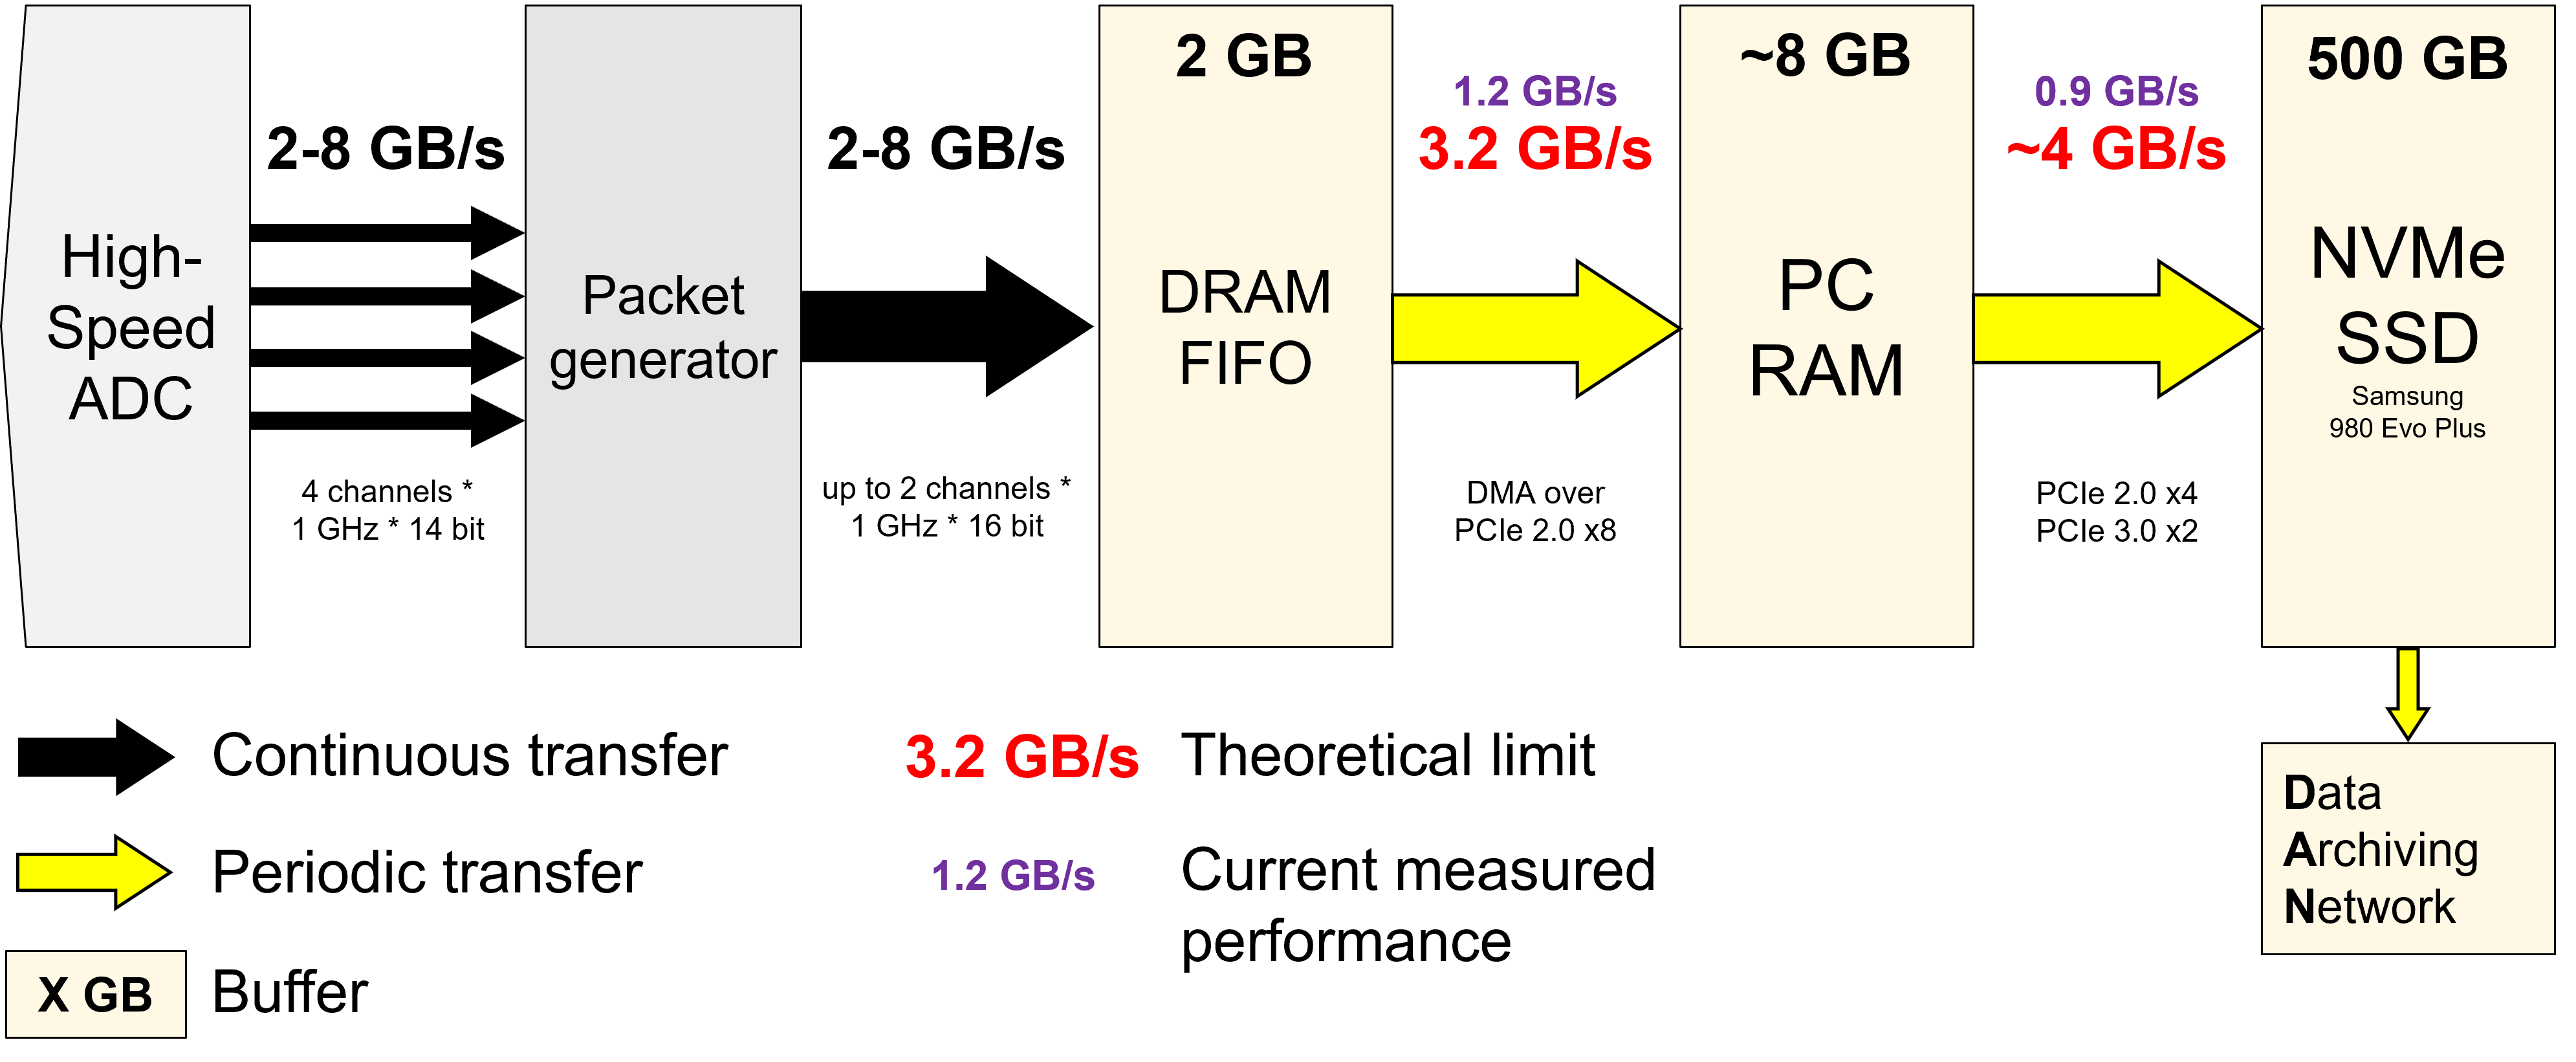
\includegraphics[width=\linewidth]{media/acquisition_buffers.png}
  \caption{Data transfer in the system}
  \label{fig:acquisition_buffers} 
\end{figure}

\subsection{PCIe interface}

A first point that can be considered for improvement is the hardware interface itself.
As of 2022 PCIe 4.0 is supported by both major CPU manufacturers.
Newest Intel processors can also make use of the PCIe 5.0 standard, 
with AMD devices to follow suit in the near future.
By upgrading the digitizer board to support PCIe 3.0 in the same x8 configuration the
theoretical throughput would double to 8 GB/s. With PCIe 4.0 it would become 16 GB/s.
Naturally, this is an issue that lies completely on the side of the board's manufacturer.
Future digitizer boards might need to target more modern interconnection standards,
to provide throughput necessary for ultra-high-speed signal acquisition.

\subsection{Direct memory access}

When using DMA, the ADQ14 splits the outgoing data into buffers.
The number and size of the buffers is configurable. Depending
on the desired application different settings should be preferred. 
To verify how the DMA buffer configuration affects transfer speed a simple
test was developed. The digitizer was programmatically configured with 
a series of varying buffer sizes and counts and used to run 20 
acquisitions, each 10 seconds long. The acquired data was not 
saved to disk, only copied in RAM.

\autoref{fig:buffer_size_speed} and \autoref{fig:buffer_count_speed}
show how the average throughput changes depending on the
configuration. In the tests with a varying buffer size 16 transfer buffers were used.
When testing the influence of the buffers count on the throughput,
the buffer size was set to 65536 bytes.
Generally larger buffers, or a higher count of buffers
provide better maximum throughput up to a certain maximum.
Increasing the size of buffers seems to provide a more consistent improvement. 
  \begin{figure}[H]
    \centering
    \begin{minipage}{.45\textwidth}
      \centering
      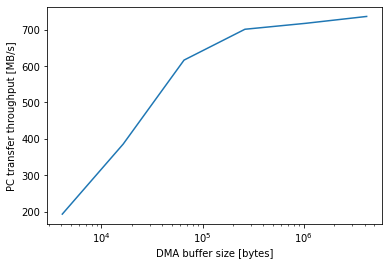
\includegraphics[width=\linewidth]{media/buffer_size_speed.png}
      \caption{DMA buffer size influencing the transfer throughput}
      \label{fig:buffer_size_speed}
    \end{minipage}%
    \hfill
    \begin{minipage}{.45\textwidth}
      \centering
      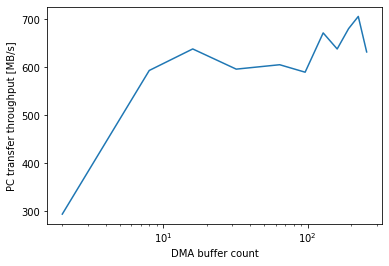
\includegraphics[width=\linewidth]{media/buffer_count_speed.png}
      \caption{DMA buffer count influencing the transfer throughput}
      \label{fig:buffer_count_speed}
    \end{minipage}
  \end{figure}

Larger buffer sizes unfortunately mean that records are packed together
into larger pages. The first record of a page will be transferred
with a significant delay in relation to its occurrence.
For example, with a record length of 1024 and a buffer size capable
of holding 10240 samples, after an event occurs, 9 more events
would have to get recorded for the first one to get transferred to the PC.


ITER's specification requires a maximum of a 5 ms delay when it comes
to transferring the acquired data to the Plasma Control System.
If the same digitizer board will also have to transfer the raw
samples for archiving and offline analysis, care will have to 
be taken when configuring these parameters. Transferring the raw signal
will require a considerable amount of bandwidth, suggesting the need for a larger
buffer size. At the same time whenever a spectrum window is finished
it should be transferred to the PC as soon as possible.
Buffers no larger than a single spectrum would work best for that.
Most likely a compromise will have to be reached experimentally.

\subsection{Acquisition software}

To control the acquisition process and handle the DMA data transfers,
a custom software GUI application was developed. The application
employs an API provided by SP Devices to interface with the digitizer board.
The Qt5 framework is used for GUI display and multiple other features.
Most importantly, the application leverages the Qt's signal/slot system 
to synchronize threaded events.


First prototypes of the application were developed with the use of PyQt, 
a library with Qt5 framework bindings for Python.
As the scope of the application grew
and the need for finer control over the performance became a priority,
the application was ported over to C++ and developed further.
\autoref{fig:qtadqscope_v1}, \autoref{fig:qtadqscope_v2} and
\autoref{fig:qtadqscope_v3} show how the application's UI 
changed with major releases.

\begin{figure}[H]
  \centering
  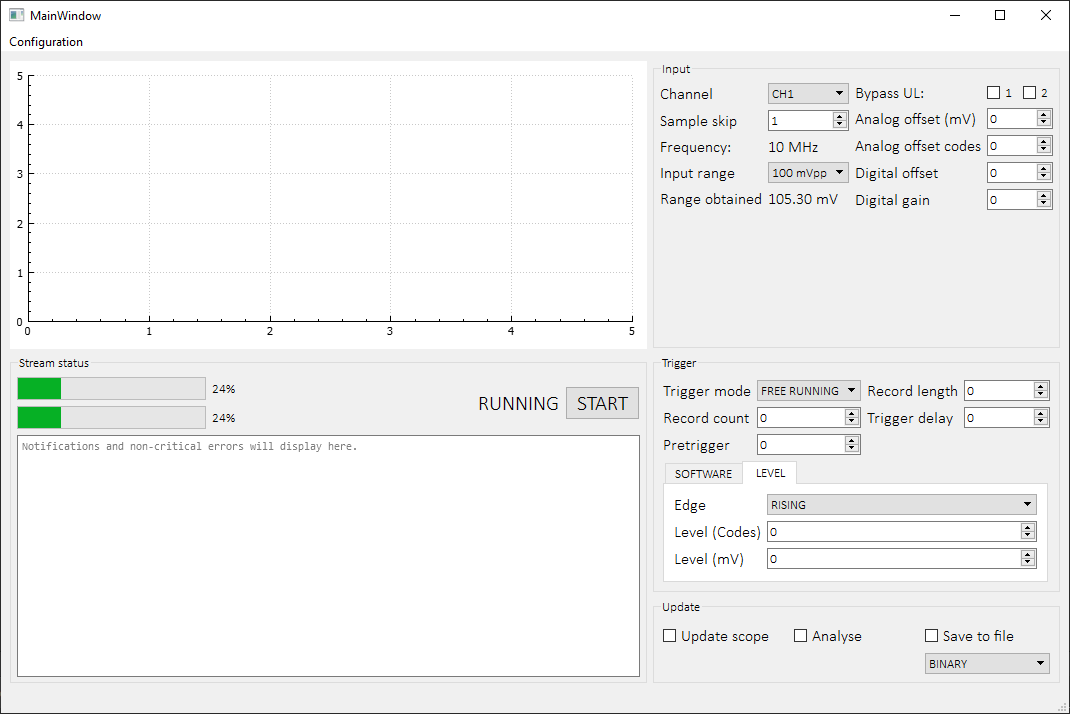
\includegraphics[width=\linewidth]{media/qtadqscope_v1.png}
  \caption{First functional acquisition software GUI written in C++}
  \label{fig:qtadqscope_v1} 
\end{figure}
\begin{figure}[H]
  \centering
  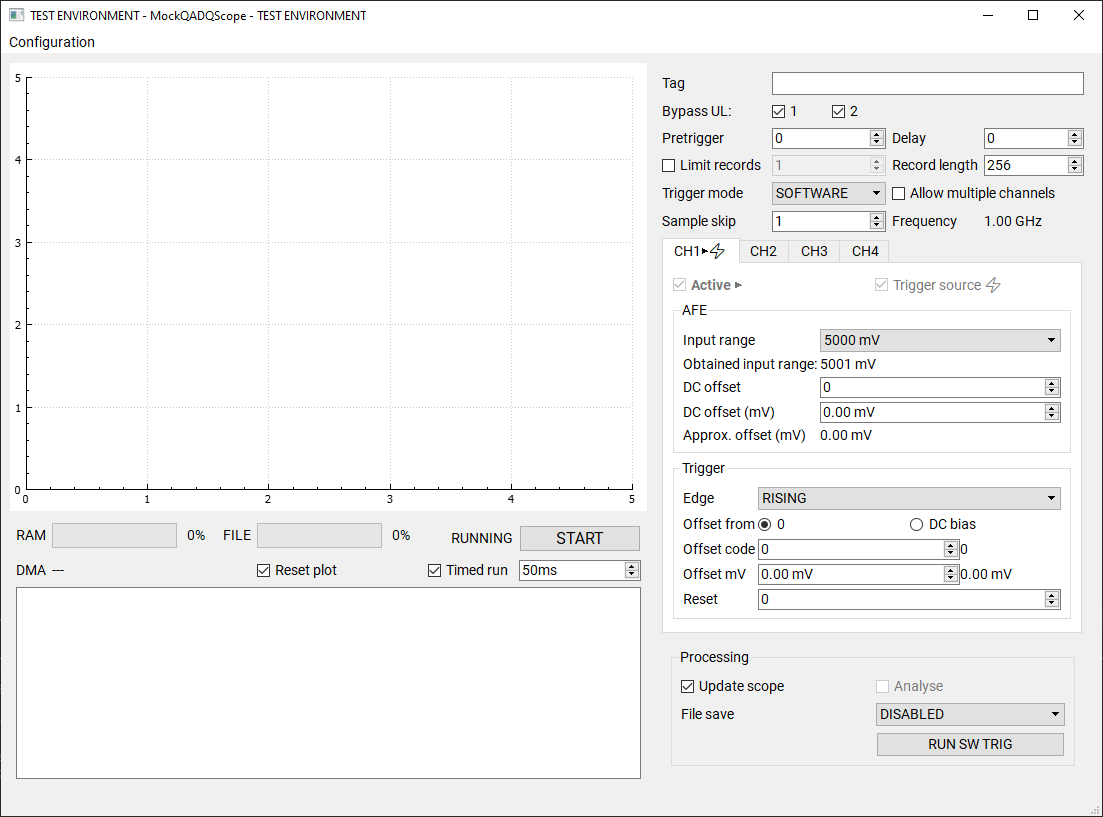
\includegraphics[width=\linewidth]{media/qtadqscope_v2.png}
  \caption{First major revision of the software application for acquisition}
  \label{fig:qtadqscope_v2} 
\end{figure}
\begin{figure}[H]
  \centering
  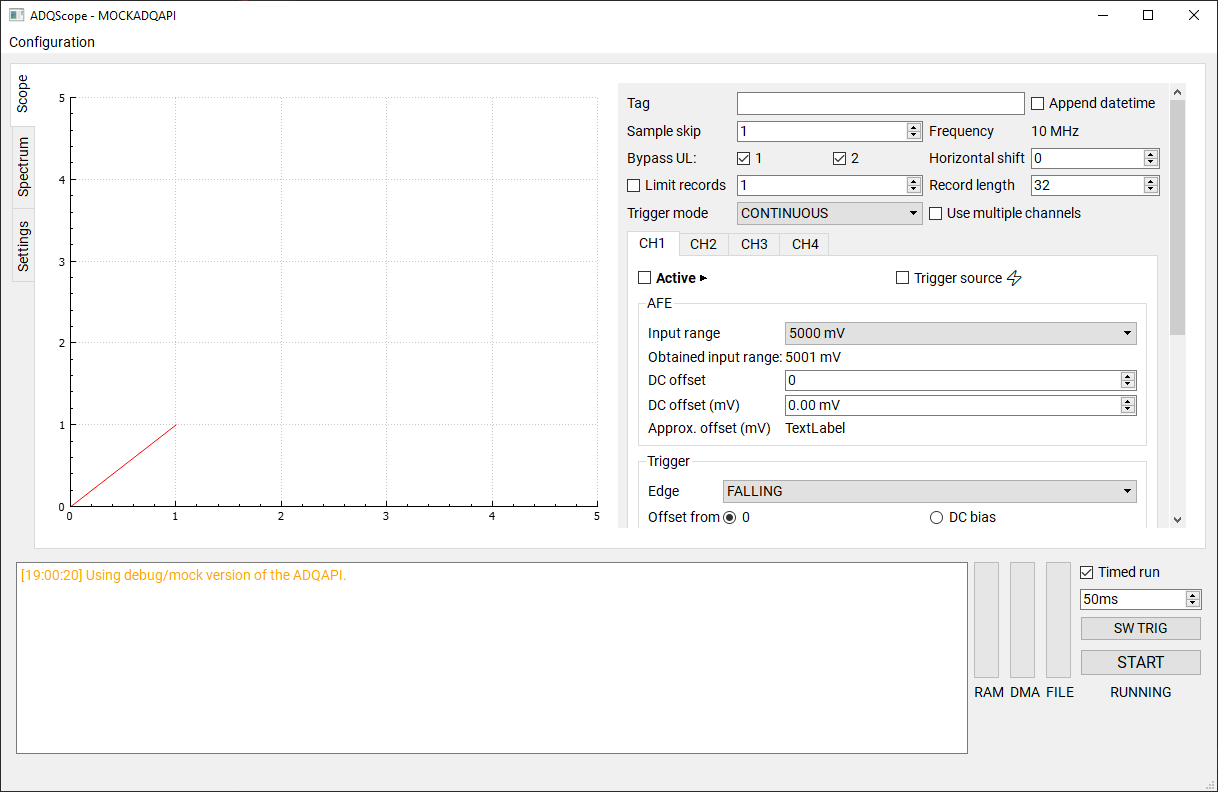
\includegraphics[width=\linewidth]{media/qtadqscope_v3.png}
  \caption{Current version of the software application for acquisition}
  \label{fig:qtadqscope_v3} 
\end{figure}
\subsubsection{Multi-threaded data transfer}

The primary thread of the software application
is used for UI display and general tasks like 
loading and saving configurations. Secondary threads
are spawned to control data acquisition and archival.
The proper operation of the worker threads
is crucial in maintaining a high data throughput.


The acquisition application was initially developed with 
the use of ADQAPI library in version 55575. That version
requires users to handle buffer processing and split the incoming
raw data into records with a custom built coroutine. \autoref{fig:adqapi_old_process}
shows the data path in version 55575. 

\begin{figure}[H]
  \centering
  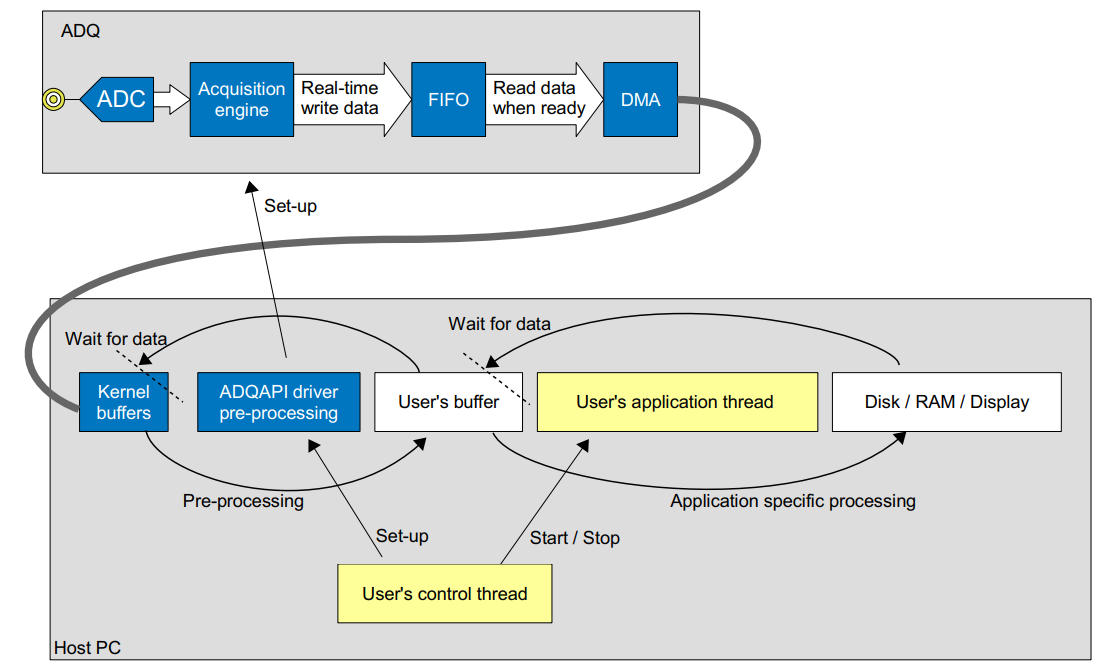
\includegraphics[width=\linewidth]{media/adqapi_old_process.png}
  \caption{Buffer transfer in ADQAPI v55575\cite{adq14_manual}}
  \label{fig:adqapi_old_process} 
\end{figure}

\autoref{fig:threads_in_old_app} shows the software acquisition pipeline in version 55575.
The maximum size of DMA buffers is limited, so as a first
step their contents is copied to another address in the PC's RAM 
to free their underlying memory.
This is done periodically in a separate worker thread.
As a DMA buffer becomes filled the worker locks one semaphore, reads its value
and copies the DMA buffer to a RAM buffer pointed to by the polled semaphore value.


Another thread polls the semaphores to get the number of filled buffers.
If a filled buffer is present it is read and processed. 
Each buffer contains a page with multiple records and their headers (metadata).
The records must be split based on the headers or a predefined configuration.
Each record is then passed on to further modules. Writing records to disk
is done in the same thread. If the records are to be displayed on screen
they must be sent over to the primary UI thread. 
Once a buffer is considered processed, the appropriate semaphore is incremented
to indicate that the buffer can be reused for writing.

\begin{figure}[H]
  \centering
  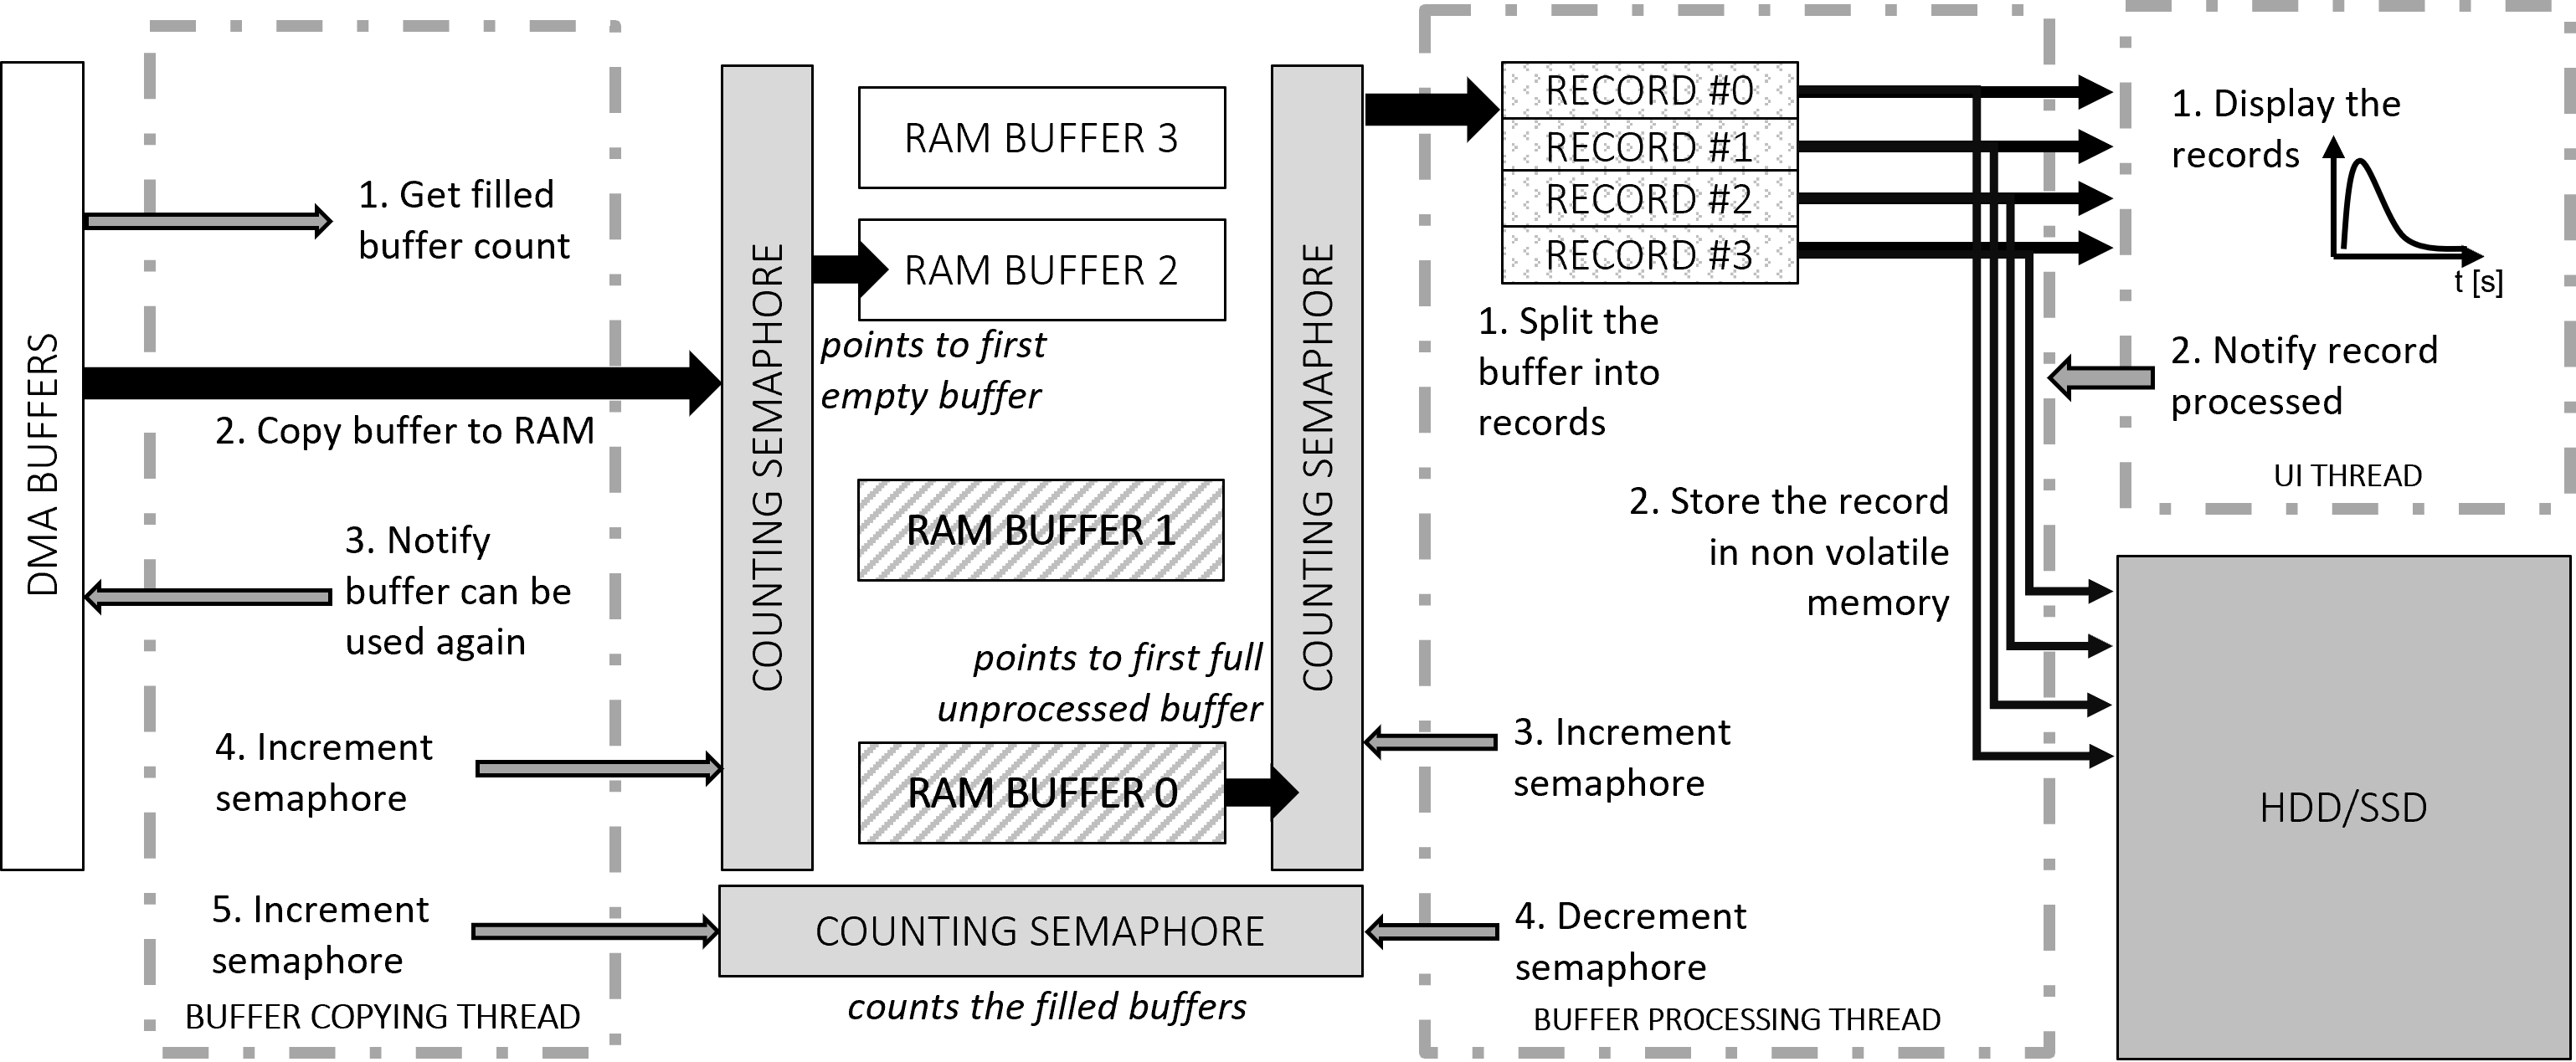
\includegraphics[width=\linewidth]{media/threads_in_old_app.png}
  \caption{Threads in the acquisition app with ADQAPI v55575}
  \label{fig:threads_in_old_app} 
\end{figure}

Plotting signals in real time is a bottleneck in the system. With a sufficiently fast
SSD drive the records can be reliably processed at a rate of up to a 1 GB/s.
The display feature, relies on a third-party library QCustomPlot which requires
the signed short integer samples output by ADQAPI
to be converted to a QVector of QDoubles (Qt5 wrappers over std::vector and double).
With as much as a few thousands of samples in each record, this is a costly operation that,
combined with the thread synchronization limits the maximum throughput to around 80 MB/s.
The scope is thus an optional feature intended for setup and debugging.


During the development of the application a new version of the ADQAPI library
was released to customers. The primary feature of ADQAPI in version 61716,
is a simplification of the buffer processing routine. The buffer copying thread
is now provided by the library. Instead of operating on raw DMA buffers,
users can choose to use the more abstract interface and work with already
split record buffers. In testing the abstraction layer was found to offer 80-90\% 
of the original performance, with the added benefit of removing a few bugs.
The new interface was implemented in the software application going forward.
\autoref{fig:threads_in_new_app} outlines the processing routine used in the more recent
version of the application.

\begin{figure}[H]
  \centering
  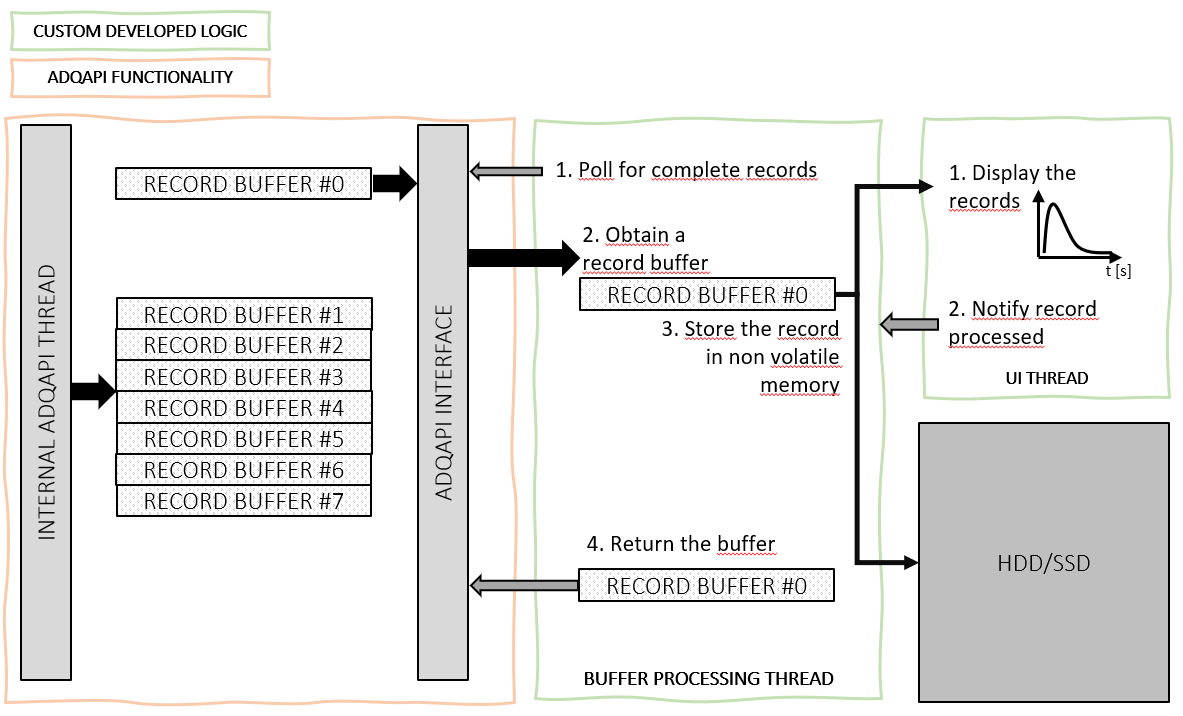
\includegraphics[width=\linewidth]{media/threads_in_new_app.png}
  \caption{Threads in the acquisition app with ADQAPI v61716}
  \label{fig:threads_in_new_app} 
\end{figure}

\subsubsection{Processing routine optimization}

A few other improvements were made to the processing routine over time.
The ADQAPI library is not thread safe. Nearly all function calls
must be done from a single synchronized thread. Accessing critical features
of the digitizer from two threads at once can crash the system.
In initial versions of the application thread safety was achieved
with a QMutex (Qt5 wrapper around std::mutex). A wrapper around the ADQAPI object
would lock the mutex before every function call. This approach enabled
the digitizer parameters to be accessed at any time, even during an acquisition.


With little input from the user the application would mostly perform
uncontested locks, which incur only a small overhead to the function calls.
The occasional contested locks could, however,
potentially cause a noticeable drop in performance.
To prevent that, the application was refactored to disable dynamic changes
to the digitizer during an acquisition. With that done, the mutex was removed
and the digitizer now exposed only a handful thread-safe methods for
starting, stopping and configuring acquisitions.
This change granted a small performance improvement of between 2-4\%
in the average throughput.


The current multithreading system relies on the use of QThreads and QObjects.
The QThread class is an interface built on top of C++ threads that 
works together with the Qt framework event queues.
In the application a worker object
that inherits from QObject is moved to a secondary QThread,
where it lives within an event loop.
This abstraction introduces an overhead when compared
to standard C++ threads, but greatly shortens the development time.
A version with a more optimized critical section is currently being developed.
Its performance will be measured once finished.

\subsubsection{Write speed optimization}

Additional upgrades were made to the disk write call itself. 
With a large amount of calls, each writing a small buffer, a drop in performance 
can be observable, when compared to lower level functions. Generally, writing 
longer chunks of data grants better performance. A simple test was performed
on the host PC to verify these facts. A series of writes was performed 
and their average write speed was noted. 
Writes were done in chunks, the size of which was changed in between tests.
\autoref{fig:chunk_bench} shows the results of this benchmark.


Initially the processing thread relied on calls to \lstinline{std::fstream::write()}.
Using \lstinline{std::fstream} introduces some abstraction over direct system calls.
The magnitude of the performance drop caused by write calls can differ 
depending on the implementation of the standard library and the computer's hardware.
To get the best possible performance the application has to be built
in release mode with the highest compiler optimization.


Typically writes are buffered, meaning that consecutive calls to a write function
actually flush to the storage medium after some buffer is filled. Until that 
the content of each write is copied over to the buffer.
Buffering can be disabled but in almost all use scenarios it causes
a massive performance drop. Fine tuning the buffer's size 
to a specific hardware and use case can lead to considerable write speed gains.


To find the best approach for the processing application, a series of simple 
write speed benchmarks were performed for varying writing methods. 
\lstinline{std::fstream} was used as the baseline and compared
to using \lstinline{FILE*} pointers with different buffer settings,
including non-buffered writes. UNIX file descriptors were also tested,
but caused up to an 80\% drop in performance, due to the lack of buffering.

  \begin{figure}[H]
    \centering
    \begin{minipage}{.45\textwidth}
      \centering
      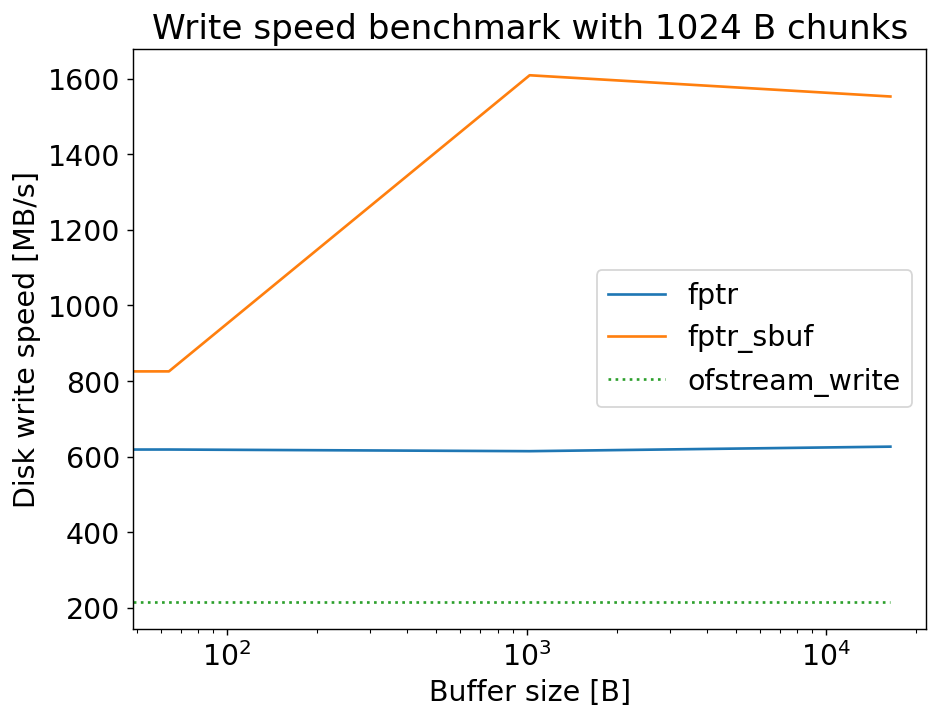
\includegraphics[width=\linewidth]{media/write_bench_1024.png}
      \caption{Write speed benchmark with a chunk size of 1024 bytes}
      \label{fig:write_bench_1024}
    \end{minipage}%
    \hfill
    \begin{minipage}{.45\textwidth}
      \centering
      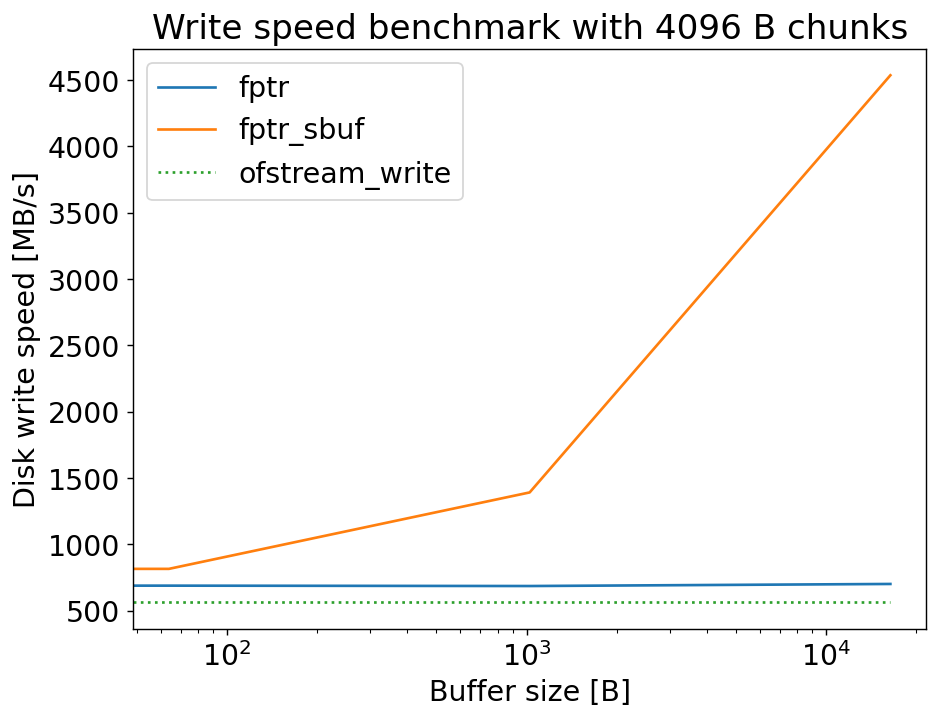
\includegraphics[width=\linewidth]{media/write_bench_4096.png}
      \caption{Write speed benchmark with a chunk size of 4096 bytes}
      \label{fig:write_bench_4096}
    \end{minipage}
  \end{figure}


  \begin{figure}[H]
    \centering
    \begin{minipage}{.45\textwidth}
      \centering
      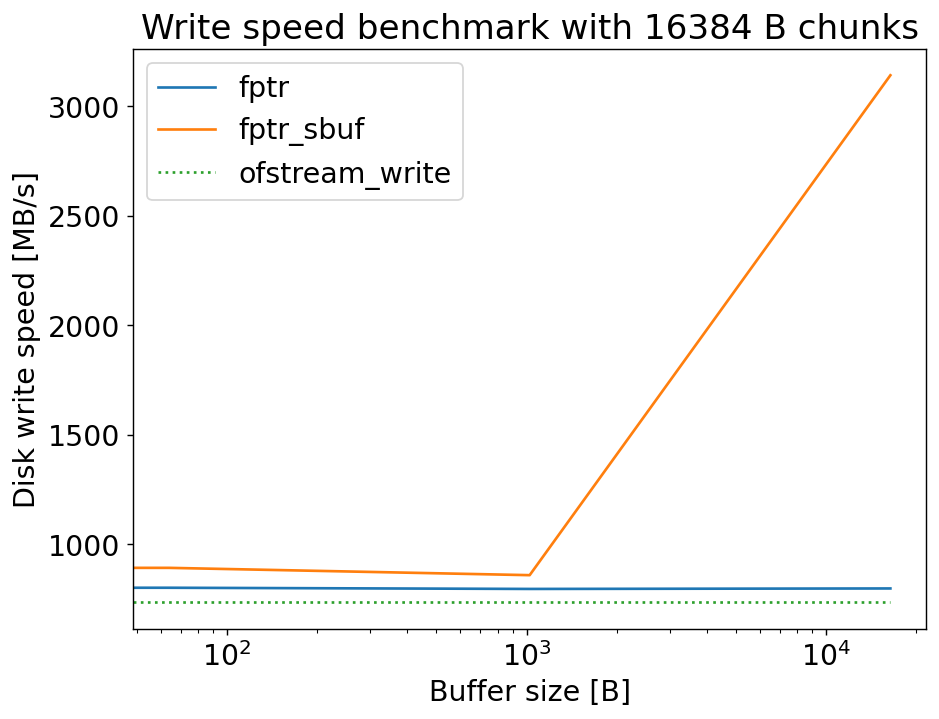
\includegraphics[width=\linewidth]{media/write_bench_16384.png}
      \caption{Write speed benchmark with a chunk size of 16384 bytes}
      \label{fig:write_bench_16384}
    \end{minipage}%
    \hfill
    \begin{minipage}{.45\textwidth}
      \centering
      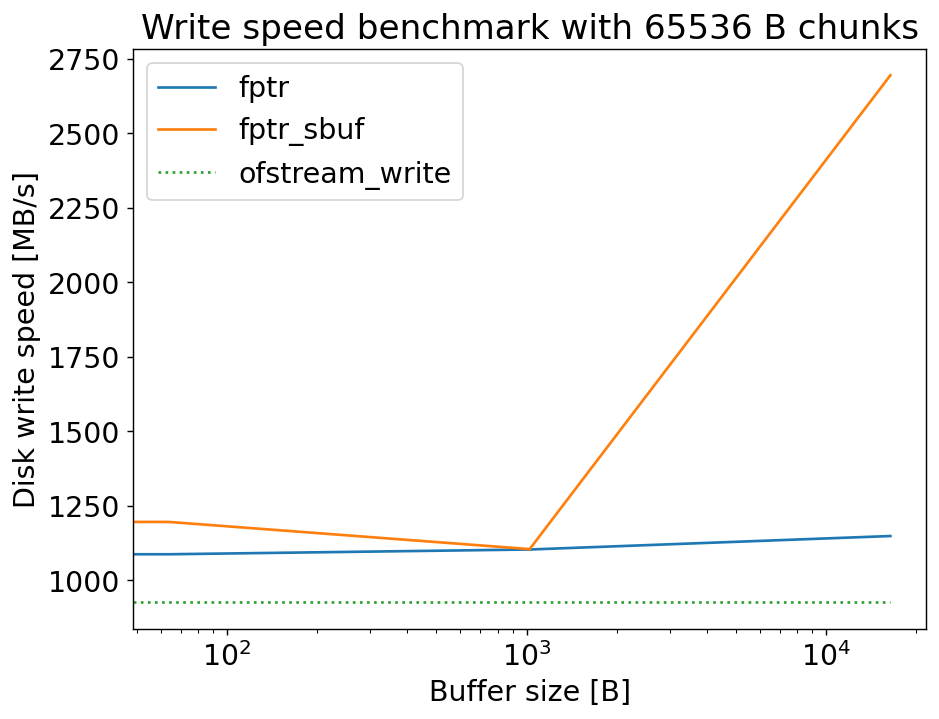
\includegraphics[width=\linewidth]{media/write_bench_65536.png}
      \caption{Write speed benchmark with a chunk size of 65536 bytes}
      \label{fig:write_bench_65536}
    \end{minipage}
  \end{figure}

  \begin{figure}[H]
    \centering
    \begin{minipage}{.45\textwidth}
      \centering
      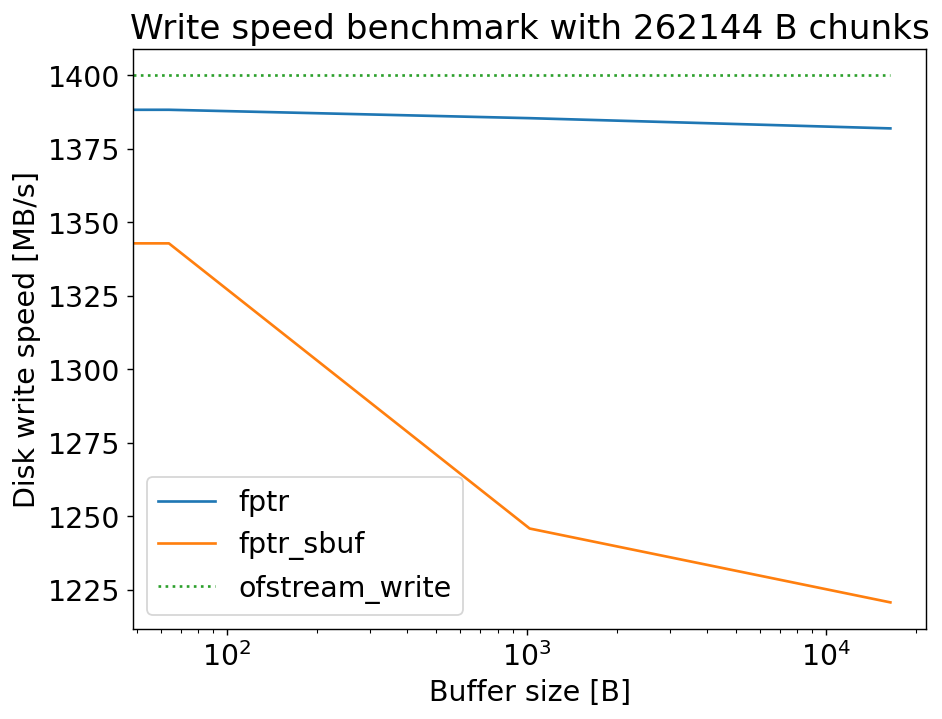
\includegraphics[width=\linewidth]{media/write_bench_262144.png}
      \caption{Write speed benchmark with a chunk size of 262144 bytes}
      \label{fig:write_bench_262144}
    \end{minipage}%
    \hfill
    \begin{minipage}{.45\textwidth}
      \centering
      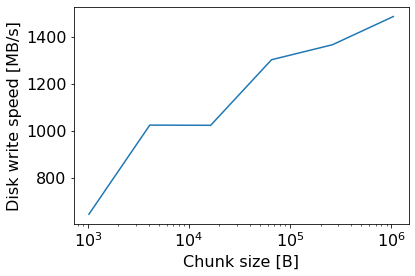
\includegraphics[width=\linewidth]{media/chunk_bench.png}
      \caption{Average write speed as a funciton of the chunk size}
      \label{fig:chunk_bench}
    \end{minipage}
  \end{figure}


The tests (\autoref{fig:write_bench_1024} - \autoref{fig:write_bench_262144})
indicate that the highest write speeds were obtained with
raw \lstinline{FILE*} pointers and user-controlled buffers (fptr\_sbuf) tuned
to the PC's SSD. In best conditions a threefold improvement
over default \lstinline{std::fstream} configuration was observed.
Letting the standard library manage the buffer
granted a stable improvement of up to 10\% in average write speed.
An equivalent drop was noticed when the size of the
chunks exceeded the size of buffers. For the time being the application 
was modified to use \lstinline{FILE*} based calls.

